Memory systems are dominant factors in large scale High Performance Computing (HPC) clusters from performance and energy consumption perspective. It also significantly contributes to the setup and operational cost of such systems. Dynamic Random Access Memory or DRAM technology has been adopted and served as the primary building blocks of main memory sub systems on the majority of computing domains including HPC. DRAM in its conventional organization (i.e. DIMMs) is struggling accommodate the exceeding memory requirements of emerging applications from different domains. This is primarily due to the fact that main memory systems and computing units are clearly separate devices and they are usually located far apart and communicate via buses that are constrained by a limited number of pins. In addition, DRAM devices usually operates in much lower frequency than the compute units (CPU/GPU). As a results, accessing the main memory for reading and writing memory blocks are expensive operations in terms of latency and energy consumption. To give a perspective, accessing data data from a DRAM device to the processing unit through the cache hierarchy takes about two orders of magnitude more energy than performing a floating point point operation in a processor. Over the years, several techniques have been adopted to complement the penalty occurring from memory operations. Several layers of cache hierarchy is introduced to reduce accesses to the main memory. Out-of-order cores are expected to continue execution while its waiting for the data from the main memory. Despite the efforts, memory access overhead continues to sustain as a major bottleneck for efficient execution of applications in HPC and other domains.

Researchers are investigating alternative solutions to keep up with the increasing memory demands from modern applications. Part of that effort focuses on using novel memory technologies based on new materials such as Phase Change Memory (PCM), Spin-Transfer-Torque Magnetic RAM (STT-MRAM), Resistive RAM (ReRAM) etc. The idea is to leverage unique properties of these memory technologies (non-volatility, endurance, no leakage current) to come up with an efficient alternative to DRAM technology. However, significant development at the cell/material level is warranted to get these memory technologies ready to attain DRAM-like performance. In addition, such extensive research and development efforts would also induce cost overhead for these technologies and it would be increasingly difficult to be commercially viable against very affordable DRAM technology.   
%be deployed and
The other approach is to change the organization of conventional memory systems using the same DRAM technology. 3D stacking of DRAM dies appears to be a convenient way to increase capacity and moving the stack closer to the CPU on the same silicon interposer greatly helps to reduce the memory access latency. Silicon interposer also allows to have denser buses (e.g. 1024 bits) between memory stack and processing unit, effectively increasing the bandwidth. Currently, High bandwidth Memory (HBM) and Hybrid Memory Cube (HMC) are the two major protocols adopting that adopt 3D stacking DRAM model.        

HMC comes with an optional logic layer beneath the stack. This logic layer can be leveraged to implement simple processing units closer to the memory, which corresponds to the technique Processing-in-memory (PIM)\footnote{Also known as Compute-in-Memory (CIM), processing-near-memory or processing-using-memory. For simplicity we refer to it as Processing-in-memory (PIM) throughout the paper.}, which builds on the idea of moving the execution of certain memory-intensive applications/kernels to the memory, instead of bringing the data to CPU for processing through expensive memory accesses. An upsurge of research activity investigating different PIM techniques indicates that it has significant potential to accelerate memory bound problems. Recent studies report significant improvements in performance and energy efficiency by adopting PIM techniques. However, these studies largely focus and analyze on the applications from Artificial Intelligence, Machine Learning, Neural Network domain along with some generic kernels. 

\begin{figure*}[t!]
\centering
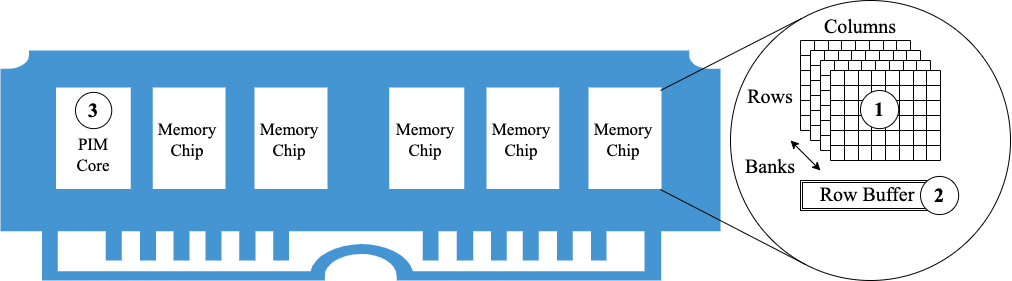
\includegraphics[width=.8\linewidth]{MEMSYS22/figures/pimcat.png}
%\vspace{.5em} 
\caption{Generic representation of a Main Memory DIMM. Processing in memory can take place at the (1) memory array, (2) row buffer or in a simple processing unit (3) closer to the banks}.
%\vspace{-1.5em} 
\label{fig:pimcat}
%\vspace{-0.6cm}    
\end{figure*}   
\looseness -1

In this paper, we perform a preliminary evaluation of HPC kernels for Processing in Memory. We select HPC benchmarks applications developed by the laboratories of US Department of Energy (DoE), identify their memory intensive kernels and analyze their suitability and performance with processing-in-memory. We also analyze key factors affecting PIM efficiency.  

The rest of the paper is organized as follows. Section 2 presents a background and related works on PIM techniques, Section 3 presents the workload characterization of target applications, Section 4 explains the experimental setup and methodologies used, Section 5 presents the results of the evaluation, and Section 6 summarizes the conclusions of the study.   


